\chapter{Simplex - Matrix Calculations}
\label{ch:simplex-matrix}

In the previous chapter we ran the simplex method through dictionaries: rewrite, pivot, repeat.  That view is good for intuition.  In this chapter we work out the \emph{linear algebra} behind it.  Every dictionary you wrote is a statement about matrices: choosing a basis means selecting an invertible submatrix $A_B$, pivoting means changing that submatrix, and the objective row of a dictionary is a vector of \emph{reduced costs} computed from $A_B^{-1}$.  Making this precise explains \emph{why} the method works, and it is how simplex is implemented in software, where solvers manipulate basis matrices rather than rewrite equations.

We proceed in two steps.  Section~\ref{sec:solutions-axb} shows how partitioning variables into basic and nonbasic sets turns $A\x = \b$ into a formula for basic solutions.  Section~\ref{sec:optimality-conditions} then rewrites the objective from the perspective of a basis, giving an algebraic certificate of optimality.

\section{Solutions to $A\x = \b$}
\label{sec:solutions-axb}
\begin{outcome}
\begin{itemize}
\item Explore how a system of equations can be rewritten via partitioning the variables
\item See how we can also partition the matrix and rewrite the equation in a new format that solves for basic variables
\item Familiarize with matrix notation
\item Define terminology of a basic solution and a basic feasible solution
\end{itemize}
\end{outcome}
We will now explore ways to represent solutions to this linear system of equations.  This is meant to give the theoretical backbone of the simplex algorithm.  

We consider a linear system

$$
A \mathbf{x} = \mathbf{b},
$$

where $A \in \mathbb{R}^{m \times n}$, $\mathbf{x} \in \mathbb{R}^n$, and $\mathbf{b} \in \mathbb{R}^m$. Explicitly,

$$
A =
\begin{bmatrix}
    a_{11} & \cdots & a_{1n} \\
    \vdots & \ddots & \vdots \\
    a_{m1} & \cdots & a_{mn}
\end{bmatrix}, \quad
\mathbf{x} =
\begin{bmatrix}
    x_1 \\
    \vdots \\
    x_n
\end{bmatrix}, \quad
\mathbf{b} =
\begin{bmatrix}
    b_1 \\
    \vdots \\
    b_m
\end{bmatrix}.
$$

\subsection*{Assumptions on $A$}

We assume:
\begin{itemize}
\item $\text{rank}(A) = m$, i.e., the rows of $A$ are linearly independent (full row rank);
\item $m \leq n$, so the system is not overdetermined.
\end{itemize}

If $A$ lacked full row rank, some equations would be redundant and removable without changing the solution set. When $m > n$, the system is typically overdetermined and inconsistent; if consistent, it can be reduced to $m \leq n$ via row operations.

Under these assumptions, $A\mathbf{x} = \mathbf{b}$ represents a system of $m$ independent equations in $n$ unknowns with a feasible (possibly infinite) solution space.

\subsubsection{Example Problem - Small Bakery}
\label{sec:bakery-problem}

A small bakery produces two products: \emph{loaves of bread} (denoted by \(x\)) and \emph{cakes} (denoted by \(y\)). Each loaf of bread contributes \$2 in profit, while each cake contributes \$3 in profit. The bakery must operate under the following daily constraints:

\begin{itemize}
    \item \textbf{Oven Time:} The total number of bread loaves and cakes baked each day cannot exceed 9, due to limited oven time. This gives the constraint:
    \[
    x + y \leq 9.
    \]
    
    \item \textbf{Flour Supply:} Bread uses more flour than cake. Each loaf uses 2 units of flour and each cake uses 1 unit. The bakery has a maximum of 16 units of flour available each day, leading to:
    \[
    2x + y \leq 16.
    \]
    
    \item \textbf{Sugar Supply:} Cakes use more sugar than bread. Each loaf uses 1 unit of sugar and each cake uses 2 units. The daily sugar supply is limited to 14 units, so:
    \[
    x + 2y \leq 14.
    \]

    \item \textbf{Non-negativity:} The bakery cannot produce a negative number of items, so:
    \[
    x \geq 0, \quad y \geq 0.
    \]
\end{itemize}

\modelhead{Model}

The bakery wants to determine how many loaves of bread (\(x\)) and cakes (\(y\)) to produce each day in order to maximize total profit. The resulting linear program is:

\begin{tcolorbox}[colback=orange!5!white, colframe=orange!75!black,    
    width=0.6\textwidth, % adjust width as desired
    box align=center, 
    title=\textbf{Original Linear Program}]
\[
\begin{aligned}
\max \quad & 2x + 3y \\
\st \quad 
& x + y \leq 9  & \text{(hours)}\\
& 2x + y \leq 16  & \text{(flour)}\\
& x + 2y \leq 14 & \text{(sugar)}\\
& x \geq 0,\; y \geq 0.
\end{aligned}
\]
\end{tcolorbox}

We begin by adding \emph{slack variables} \( s_1, s_2, s_3 \) to convert the inequalities to equalities:

\begin{tcolorbox}[colback=gray!5!white, colframe=gray!75!black,    
    width=0.6\textwidth, % adjust width as desired
    box align=center, 
    title=\textbf{Standard Form}]
\[
\begin{aligned}
\max \quad & 2x + 3y \\
\st \quad 
&x + y + s_1 = 9 \quad &\text{(hours)} \\
&2x + y + s_2 = 16 \quad &\text{(flour)} \\
&x + 2y + s_3 = 14 \quad &\text{(sugar)} \\
&x, y, s_1, s_2, s_3 \geq 0
\end{aligned}
\]
\end{tcolorbox}

It will be useful to also understand standard form from the matrix perspective.

\begin{tcolorbox}[colback=gray!5!white, colframe=gray!75!black,    
    width=0.8\textwidth, % adjust width as desired
    box align=center, 
    title=\textbf{Matrix-Vector Standard Form}]
\noindent In matrix-vector notation, define:
\[
\mathbf{x} = 
\begin{bmatrix}
x \\
y \\
s_1 \\
s_2 \\
s_3
\end{bmatrix},
\quad
\mathbf{c} =
\begin{bmatrix}
2 \\
3 \\
0 \\
0 \\
0
\end{bmatrix},
\quad
A =
\begin{bmatrix}
1 & 1 & 1 & 0 & 0 \\
2 & 1 & 0 & 1 & 0 \\
1 & 2 & 0 & 0 & 1
\end{bmatrix},
\quad
\mathbf{b} =
\begin{bmatrix}
9 \\
16 \\
14
\end{bmatrix}
\]

\bigskip

\noindent The standard form linear program is then:
\[
\begin{aligned}
\max \quad & \mathbf{c}^\top \mathbf{x} \\
\st \quad & A\mathbf{x} = \mathbf{b}, \\
& \mathbf{x} \geq \mathbf{0}
\end{aligned}
\]

\end{tcolorbox}

\subsection*{Submatrix Notation}
We extract submatrices of \( A \) by selecting columns corresponding to specific variable sets.  
For a set \( I \), we let \( A_I \) denote the submatrix of \( A \) corresponding to the columns in \( I \).

\bigskip

\[
\begin{array}{c}
\begin{array}{ccccc}
\scriptstyle x & \scriptstyle y & \scriptstyle s_1 & \scriptstyle s_2 & \scriptstyle s_3
\end{array} \\
\left[
\begin{array}{>{\columncolor{yellow}}c c c c c}
1 & 1 & 1 & 0 & 0 \\
2 & 1 & 0 & 1 & 0 \\
1 & 2 & 0 & 0 & 1
\end{array}
\right]
\end{array}
\quad
\Rightarrow
\quad
A_{\{x\}} =
\begin{bmatrix}
1 \\
2 \\
1
\end{bmatrix}
\]

\bigskip

\[
\begin{array}{c}
\begin{array}{ccccc}
\scriptstyle x & \scriptstyle y & \scriptstyle s_1 & \scriptstyle s_2 & \scriptstyle s_3
\end{array} \\
\left[
\begin{array}{c>{\columncolor{cyan}}c c >{\columncolor{cyan}}c c}
1 & 1 & 1 & 0 & 0 \\
2 & 1 & 0 & 1 & 0 \\
1 & 2 & 0 & 0 & 1
\end{array}
\right]
\end{array}
\quad
\Rightarrow
\quad
A_{\{y, s_2\}} =
\begin{bmatrix}
1 & 0 \\
1 & 1 \\
2 & 0
\end{bmatrix}
\]
\bigskip

\[
\begin{array}{c}
\begin{array}{ccccc}
\scriptstyle x & \scriptstyle y & \scriptstyle s_1 & \scriptstyle s_2 & \scriptstyle s_3
\end{array} \\
\left[
\begin{array}{c c >{\columncolor{orange}}c >{\columncolor{orange}}c >{\columncolor{orange}}c}
1 & 1 & 1 & 0 & 0 \\
2 & 1 & 0 & 1 & 0 \\
1 & 2 & 0 & 0 & 1
\end{array}
\right]
\end{array}
\quad
\Rightarrow
\quad
A_{\{s_1, s_2, s_3\}} =
\begin{bmatrix}
1 & 0 & 0 \\
0 & 1 & 0 \\
0 & 0 & 1
\end{bmatrix}
\]

\bigskip

\begin{align*}
A\mathbf{x}
&=
\begin{bmatrix}
1 & 1 & 1 & 0 & 0 \\
2 & 1 & 0 & 1 & 0 \\
1 & 2 & 0 & 0 & 1
\end{bmatrix}
\begin{bmatrix}
x \\ y \\ s_1 \\ s_2 \\ s_3
\end{bmatrix}
=
\begin{bmatrix}
1x + 1y + 1s_1 \\
2x + 1y + 1s_2 \\
1x + 2y + 1s_3
\end{bmatrix} \\
&=
\underbrace{
\begin{bmatrix}
1 & 1 \\
2 & 1 \\
1 & 2
\end{bmatrix}
\begin{bmatrix}
x \\ y
\end{bmatrix}
}_{A_{\{x,y\}} (x, y)}
+
\underbrace{
\begin{bmatrix}
1 & 0 & 0 \\
0 & 1 & 0 \\
0 & 0 & 1
\end{bmatrix}
\begin{bmatrix}
s_1 \\ s_2 \\ s_3
\end{bmatrix}
}_{A_{\{s_1,s_2,s_3\}} (s_1, s_2, s_3)}
\end{align*}

\bigskip

\begin{align*}
A\mathbf{x}
&=
\underbrace{
\begin{bmatrix}
1 & 1 & 0 \\
2 & 1 & 1 \\
1 & 2 & 0
\end{bmatrix}
\begin{bmatrix}
x \\ y \\ s_2
\end{bmatrix}
}_{A_{\{x, y, s_2\}} (x, y, s_2)}
+
\underbrace{
\begin{bmatrix}
1 & 0 \\
0 & 0 \\
0 & 1
\end{bmatrix}
\begin{bmatrix}
s_1 \\ s_3
\end{bmatrix}
}_{A_{\{s_1, s_3\}} (s_1, s_3)}
=
\begin{bmatrix}
9 \\ 16 \\ 14
\end{bmatrix}
\end{align*}

\bigskip

This implies:

\begin{align*}
A_{\{x, y, s_2\}} 
\begin{bmatrix}
x \\ y \\ s_2
\end{bmatrix}
&=
\begin{bmatrix}
9 \\ 16 \\ 14
\end{bmatrix}
-
A_{\{s_1, s_3\}}
\begin{bmatrix}
s_1 \\ s_3
\end{bmatrix}
\end{align*}

\bigskip

So,

\begin{align*}
\begin{bmatrix}
x \\ y \\ s_2
\end{bmatrix}
&=
A_{\{x, y, s_2\}}^{-1}
\left(
\begin{bmatrix}
9 \\ 16 \\ 14
\end{bmatrix}
-
A_{\{s_1, s_3\}}
\begin{bmatrix}
s_1 \\ s_3
\end{bmatrix}
\right)
\end{align*}

\subsection{Partitioning the Variables}

In solving the system \( A\x =\b\) in the context of linear programming, we introduce the concept of \textbf{partitioning the variables}. This approach is essential in the Simplex Method for identifying and analyzing basic solutions.

\begin{definition}{Basis}{}
Given a matrix $A$ of full row rank $m$, a \emph{basis} $B$ is an index set of $m$ of the $n$ columns such that the corresponding $m$ columns of the matrix $A$ are linearly independent.  We then form the submatrix $A_B$ that contains only those columns of $A$. 

 The remaining \( n - m \) columns are referred to as the \emph{nonbasic} columns, which form the matrix \( A_N \). 
 \end{definition}
 
 Given a basis $B$ and the nonbasic set $N$, this partitions the variable vector \( \x \) into two sets:
\[
\x =
\begin{bmatrix}
    \x_B \\ \x_N
\end{bmatrix},
\]
where:
\begin{itemize}
\item  \( \x_B \) consists of the \textbf{basic variables}, associated with the basis matrix \( A_B \),
\item\( \x_N \) consists of the \textbf{nonbasic variables}, associated with the nonbasic matrix \( A_N \).
\end{itemize}

Rewriting the system \( A\x =\b\) in terms of these partitions gives:
\begin{equation}
A_B \x_B + A_N \x_N = b.
\end{equation}

If the basis matrix \( A_B \) is invertible, we can express \( \x_B \) in terms of \( \x_N \):
\begin{equation}
\x_B = A_B^{-1}\b- A_B^{-1} A_N \x_N.
\end{equation}

\begin{definition}{Basic solution and Basic Feasible Solution (BFS)}{}
A \textbf{basic solution} is obtained by setting \( \x_N = 0 \), yielding:
\begin{equation}
\x_B = A_B^{-1} \b, \quad \x_N = 0.
\end{equation}

A \textbf{basic feasible solution} (BFS) is a basic solution that satisfies the nonnegativity constraint \( \x_B \geq \0 \), ensuring that all basic variables are nonnegative.
\end{definition}
\subsubsection*{Example 1: A 3-variable, 2-equation System}

Consider the following system:
\[
\begin{aligned}
    x_1 + 2x_2 + x_3 &= 4, \\
    3x_1 + x_2 + 2x_3 &= 5.
\end{aligned}
\]
Here, the matrix \( A \) and the variable vector \( x \) are:
\[
A =
\begin{bmatrix}
    1 & 2 & 1 \\
    3 & 1 & 2
\end{bmatrix}, \quad
x =
\begin{bmatrix}
    x_1 \\ x_2 \\ x_3
\end{bmatrix}, \quad
b =
\begin{bmatrix}
    4 \\ 5
\end{bmatrix}.
\]
Selecting \(B= \{1, 2\} \) as the basis, the corresponding submatrix is:
\[
A_B =
\begin{bmatrix}
    1 & 2 \\
    3 & 1
\end{bmatrix}, \quad A_N =
\begin{bmatrix}
    1 \\
    2
\end{bmatrix}.
\]
If \( A_B \) is invertible, we compute:
\[
A_B^{-1} =
\begin{bmatrix}
    -1/5 & 2/5 \\
    3/5 & -1/5
\end{bmatrix}.
\]
Setting \( x_3 = 0 \) (i.e., \( \x_N = 0 \)), we solve for \( \x_B \):
\[
x_B = A_B^{-1}\b=
\begin{bmatrix}
    -1/5 & 2/5 \\
    3/5 & -1/5
\end{bmatrix}
\begin{bmatrix}
    4 \\ 5
\end{bmatrix}
=
\begin{bmatrix}
    6/5 \\
    7/5
\end{bmatrix}.
\]
Since \( \x_B \geq 0 \), this is a \textbf{basic feasible solution}.

\subsubsection*{Example 2: A System with Slack Variables}

Consider a linear program in inequality form:
\[
\begin{aligned}
    x_1 + 3x_2 &\leq 6, \\
    2x_1 + x_2 &\leq 4.
\end{aligned}
\]
We introduce slack variables \( s_1, s_2 \geq 0 \) to convert inequalities into equalities:
\[
\begin{aligned}
    x_1 + 3x_2 + s_1 &= 6, \\
    2x_1 + x_2 + s_2 &= 4.
\end{aligned}
\]
The augmented system has:
\[
A =
\begin{bmatrix}
    1 & 3 & 1 & 0 \\
    2 & 1 & 0 & 1
\end{bmatrix}, \quad
x =
\begin{bmatrix}
    x_1 \\ x_2 \\ s_1 \\ s_2
\end{bmatrix}, \quad
b =
\begin{bmatrix}
    6 \\ 4
\end{bmatrix}.
\]
Choosing the slack variables as the basis (\(B= \{s_1, s_2\} \)), the basis matrix is:
\[
A_B =
\begin{bmatrix}
    1 & 0 \\
    0 & 1
\end{bmatrix}, \quad A_N =
\begin{bmatrix}
    1 & 3 \\
    2 & 1
\end{bmatrix}.
\]
Since \( A_B \) is the identity matrix, its inverse is itself, and we obtain:
\[
\x_B = A_B^{-1}\b= 
\begin{bmatrix}
    6 \\ 4
\end{bmatrix}, \quad \x_N = 0.
\]
Since \( \x_B \geq 0 \), this is a \textbf{basic feasible solution}.

\subsection{Another Example}

To convert the given problem into standard form, we introduce \textbf{slack variables} \( s_1, s_2 \) to convert the inequalities into equalities.

\[
\begin{aligned}
    \max \quad & 2 x_1 + 5 x_2 \\
    \st \quad 
    & x_1 + 2x_2 + s_1 = 16, \\
    & 5x_1 + 3x_2 + s_2 = 45, \\
    & x_1, x_2, s_1, s_2 \geq 0.
\end{aligned}
\]

Now the system is in standard form:
\[
\begin{bmatrix}
    1 & 2 & 1 & 0 \\
    5 & 3 & 0 & 1
\end{bmatrix}
\begin{bmatrix}
    x_1 \\ x_2 \\ s_1 \\ s_2
\end{bmatrix}
=
\begin{bmatrix}
    16 \\ 45
\end{bmatrix}, \quad x_1, x_2, s_1, s_2 \geq 0.
\]

\subsection{Selecting and Evaluating Different Bases}
\label{sec:three-bases}

A basis consists of any two linearly independent columns from \( A \). We select three different bases:
\begin{itemize}
\item  Basis 1: \(B= \{x_1, x_2\} \) (Feasible)
The basis matrix is:
\[
A_B =
\begin{bmatrix}
    1 & 2 \\
    5 & 3
\end{bmatrix}.
\]
Computing \( A_B^{-1} \):
\[
A_B^{-1} =
\frac{1}{(1)(3) - (2)(5)}
\begin{bmatrix}
    3 & -2 \\
    -5 & 1
\end{bmatrix}
=
\frac{1}{3 - 10}
\begin{bmatrix}
    3 & -2 \\
    -5 & 1
\end{bmatrix}
=
\frac{1}{-7}
\begin{bmatrix}
    3 & -2 \\
    -5 & 1
\end{bmatrix}
=
\begin{bmatrix}
    -3/7 & 2/7 \\
    5/7 & -1/7
\end{bmatrix}.
\]
Computing the basic solution:
\[
\x_B = A_B^{-1}\b=
\begin{bmatrix}
    -3/7 & 2/7 \\
    5/7 & -1/7
\end{bmatrix}
\begin{bmatrix}
    16 \\ 45
\end{bmatrix}
=
\begin{bmatrix}
    (-3/7)(16) + (2/7)(45) \\
    (5/7)(16) + (-1/7)(45)
\end{bmatrix}
\]
\[
=
\begin{bmatrix}
    -48/7 + 90/7 \\
    80/7 - 45/7
\end{bmatrix}
=
\begin{bmatrix}
    42/7 \\
    35/7
\end{bmatrix}
=
\begin{bmatrix}
    6 \\ 5
\end{bmatrix}.
\]
Since \( \x_B = (6,5) \) contains no negative values, this basis indeed yields a \textbf{feasible solution}.

\item  Basis 2: \(B= \{x_1, s_2\} \) (Infeasible)
The basis matrix (the columns of \( x_1 \) and \( s_2 \)) is:
\[
A_B =
\begin{bmatrix}
    1 & 0 \\
    5 & 1
\end{bmatrix}.
\]
Computing \( A_B^{-1} \):
\[
A_B^{-1} =
\frac{1}{(1)(1) - (0)(5)}
\begin{bmatrix}
    1 & 0 \\
    -5 & 1
\end{bmatrix}
=
\begin{bmatrix}
    1 & 0 \\
    -5 & 1
\end{bmatrix}.
\]
Computing the basic solution:
\[
\x_B = \begin{bmatrix} x_1 \\ s_2 \end{bmatrix} = A_B^{-1}\b=
\begin{bmatrix}
    1 & 0 \\
    -5 & 1
\end{bmatrix}
\begin{bmatrix}
    16 \\ 45
\end{bmatrix}
=
\begin{bmatrix}
    (1)(16) + (0)(45) \\
    (-5)(16) + (1)(45)
\end{bmatrix}
=
\begin{bmatrix}
    16 \\
    -80 + 45
\end{bmatrix}
=
\begin{bmatrix}
    16 \\ -35
\end{bmatrix}.
\]
Since \( s_2 = -35 < 0 \), this basis is \textbf{infeasible}.  The corresponding point is \( (x_1, x_2) = (16, 0) \), which violates the constraint \( 5x_1 + 3x_2 \leq 45 \).

\item  Basis 3: \(B= \{s_1, s_2\} \) (Feasible)
The basis matrix is:
\[
A_B =
\begin{bmatrix}
    1 & 0 \\
    0 & 1
\end{bmatrix}.
\]
Since this is the identity matrix, its inverse is itself. Thus, the basic solution is:
\[
\x_B = \begin{bmatrix} s_1 \\ s_2 \end{bmatrix} = A_B^{-1}\b=
\begin{bmatrix}
    16 \\ 45
\end{bmatrix}.
\]
Since all basic variables are nonnegative, this is a \textbf{feasible solution}.
\end{itemize}

Figure~\ref{fig:matrix-bases-geometry} shows where these three basic solutions sit relative to the feasible region.

\begin{figure}[h!]
\begin{center}
% Feasible region for max 2x1+5x2 s.t. x1+2x2<=16, 5x1+3x2<=45, x1,x2>=0.
% Vertices: (0,0), (9,0), (6,5), (0,8).  Basic solutions from the three bases:
% B={x1,x2} -> (6,5), B={s1,s2} -> (0,0), B={x1,s2} -> (16,0) infeasible.
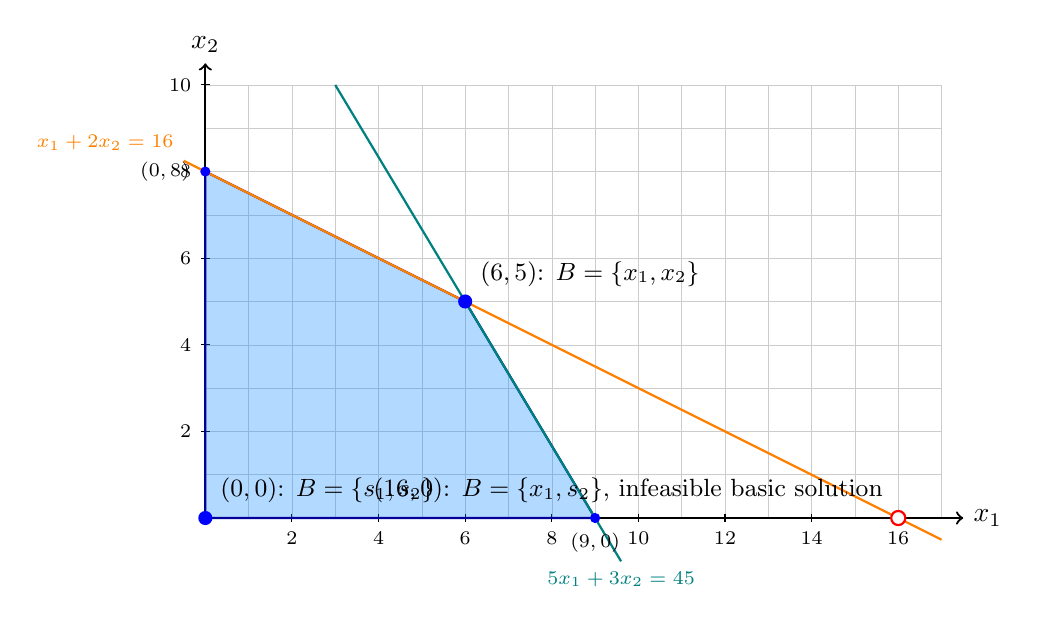
\begin{tikzpicture}[scale=0.55]
    % Grid and axes
    \draw[gray!40, very thin, step=1] (0,0) grid (17,10);
    \draw[->, thick] (0,0) -- (17.5,0) node[right] {$x_1$};
    \draw[->, thick] (0,0) -- (0,10.5) node[above] {$x_2$};
    \foreach \x in {2,4,...,16} \draw (\x,0.1) -- (\x,-0.1) node[below] {\scriptsize \x};
    \foreach \y in {2,4,...,10} \draw (0.1,\y) -- (-0.1,\y) node[left] {\scriptsize \y};

    % Feasible region
    \fill[blue!50!cyan, opacity=0.3] (0,0) -- (9,0) -- (6,5) -- (0,8) -- cycle;
    \draw[blue!60!black, thick] (0,0) -- (9,0) -- (6,5) -- (0,8) -- cycle;

    % Constraint boundaries
    \draw[orange, thick] (-0.5,8.25) node[above left] {\scriptsize $x_1+2x_2=16$} -- (17,-0.5);
    \draw[teal, thick] (3,10) -- (9.6,-1) node[below] {\scriptsize $5x_1+3x_2=45$};

    % Remaining vertices of the region
    \node[fill=blue,circle,inner sep=1.3pt,label={below:\scriptsize $(9,0)$}] at (9,0) {};
    \node[fill=blue,circle,inner sep=1.3pt,label={left:\scriptsize $(0,8)$}] at (0,8) {};

    % Basic solutions from the three bases
    \node[fill=blue,circle,inner sep=1.8pt,
        label={above right:\small $(6,5)$: $B=\{x_1,x_2\}$}] at (6,5) {};
    \node[fill=blue,circle,inner sep=1.8pt,
        label={above right:\small $(0,0)$: $B=\{s_1,s_2\}$}] at (0,0) {};
    \node[draw=red,thick,circle,fill=white,inner sep=1.8pt,
        label={above left:\small $(16,0)$: $B=\{x_1,s_2\}$, infeasible basic solution}] at (16,0) {};
\end{tikzpicture}
\end{center}
\caption{The three bases of this subsection, seen geometrically.  Each basis fixes the nonbasic variables at zero, which places the basic solution at the intersection of two constraint boundaries.  Bases $\{x_1,x_2\}$ and $\{s_1,s_2\}$ give basic \emph{feasible} solutions at the vertices $(6,5)$ and $(0,0)$ (filled dots).  Basis $\{x_1,s_2\}$ gives the basic solution $(16,0)$ (open dot), the intersection of the $x_1$-axis ($x_2=0$) with the boundary $x_1+2x_2=16$ ($s_1=0$); it violates $5x_1+3x_2\le 45$, so it is an infeasible basic solution and lies outside the region.}
\label{fig:matrix-bases-geometry}
\end{figure}

\section{Optimality Conditions}
\label{sec:optimality-conditions}
\begin{outcome}
\begin{itemize}
\item Define reduced costs at a basic feasible solution
\item Establish optimality conditions via the reduced costs
\end{itemize}
\end{outcome}
The objective function of the linear program is given by:
    \[
    z = \c^\top \x.
    \]
    Substituting the partitioned variables \( \x_B \) and \( \x_N \),
    \[
    z =\c_B^\top \x_B +\c_N^\top \x_N.
    \]
    Expressing \( \x_B \) in terms of \( \x_N \), using the basic solution \( \x_B = A_B^{-1}\b- A_B^{-1} A_N \x_N \), we rewrite the objective function as:
    \begin{equation}
    z =\c_B^\top (A_B^{-1}\b- A_B^{-1} A_N \x_N) +\c_N^\top \x_N.
    \end{equation}
    Expanding and regrouping terms:
    \begin{equation}
    z =\c_B^\top A_B^{-1}\b+  (\c_N^\top -\c_B^\top A_B^{-1} A_N )\x_N.
    \end{equation}
    \begin{definition}{Reduced Costs}{}
    The term \(\c_N^\top -\c_B^\top A_B^{-1} A_N \) represents the \emph{reduced costs}.  
    
    This is explained as the objective rewritten from the viewpoint of a basic feasible solution. In particular, these are the coefficients on the non-basic variables.
\end{definition}
    

The system is rewritten as the dictionary form at basis $B$ as in the following definition.

\begin{definition}{Revised Simplex Dictionary at basis $B$}{}
The \emph{revised simplex dictionary} at a basis $B$ is 
\begin{equation}
\label{eq:dictionary-general}
\begin{aligned}
\max \quad & \mathbf{c}_B^\top A_B^{-1}\mathbf{b} + (\mathbf{c}_N^\top -  \mathbf{c}_B^\top A_B^{-1}A_N)\mathbf{x}_N\\
\st \quad & 
 \mathbf{x}_B 
\;=\;
A_B^{-1}\,\mathbf{b}
\;-\;
A_B^{-1} \,A_N\,\mathbf{x}_N.\\
& \mathbf{x} \geq 0
\end{aligned}
\end{equation}
\end{definition}

Here is an example: the same linear program written first at the slack basis and then at the basis $\{x, y\}$.

\[
\begin{aligned}
\max\quad & 2x + y \\
\st\quad & s_1 = 23 - 3x - y,\\ 
& s_2 = 45 - 5x - 3y,\\ 
& x, y, s_1, s_2 \ge 0.
\end{aligned}
\]

\[
\begin{aligned}
\max\quad & 17 - 0.25s_1 - 0.25s_2 \\
\st\quad & x = 6 - 0.75s_1 + 0.25s_2,\\ 
& y = 5 + 1.25s_1 - 0.75s_2,\\ 
& x, y, s_1, s_2 \ge 0.
\end{aligned}
\]

\begin{theorem}{Optimality Condition in Simplex Method}{}

    Given a linear program in standard form:
    \[
    \max \; \c^\top \x \quad \st \quad A \x = b, \quad \x \geq 0,
    \]
    let \(B\) be a basis corresponding to a basic feasible solution \( \x_B = A_B^{-1}\b\), with nonbasic variables \( \x_N = 0 \).

    If all reduced costs satisfy:
    \[
   \c_N^\top -\c_B^\top A_B^{-1} A_N \leq 0,
    \]
    then the current basic feasible solution is optimal.
\end{theorem}
\begin{proof}
Let $\bar \x = (\bar \x_B, \bar \x_N) = (A_B^{-1}\b, \0)$.

    If all reduced costs are nonpositive, i.e.,
    \[
   \c_N^\top -\c_B^\top A_B^{-1} A_N \leq 0,
    \]
    then for any feasible choice of \( \x_N \geq 0 \), 
    we have
    \begin{align}
    \c^\top \x &= \c_B^\top A_B^{-1}\b+  (\c_N^\top -\c_B^\top A_B^{-1} A_N )\x_N\\
    &= \c^\top \bar \x +  (\c_N^\top -\c_B^\top A_B^{-1} A_N )\x_N\\
    & \leq \c^\top \bar \x,
    \end{align}
    where the last line follows since $(\c_N^\top -\c_B^\top A_B^{-1} A_N ) \leq 0$ and $\x_N \geq 0$.
    
    Thus, $\bar \x$ is an optimal solution!
\end{proof}

\label{par:matrix-sign-conventions}%
A note on sign conventions.  The three treatments of the simplex method in this book state the same optimality test in three ways.  In the dictionary form of Chapter~\ref{ch:simplex-dictionary}, we improve the solution by increasing a nonbasic variable with a \emph{positive} coefficient in the objective row, and we stop when there is none.  The theorem above says the same thing in matrix language: those coefficients are the reduced costs $\c_N^\top -\c_B^\top A_B^{-1} A_N$, and the solution is optimal once they are all $\leq 0$.  In the tableau form of Chapter~\ref{ch:simplex-tableau}, the objective is stored as the equation $z - \c^\top\x = 0$, which flips the signs of these coefficients, so there you look for \emph{negative} $z$-row entries and stop when every entry is nonnegative.  All three are the same test.

\begin{example}{Verifying Optimality Using Reduced Costs}{}

We aim to verify that the basic feasible solutions \( (6,5) \) and \( (0,8) \) are optimal for the following linear program:

\[
\begin{aligned}
    \max \quad & 2 x_1 + 5 x_2 \\
    \st \quad 
    & x_1 + 2x_2 + s_1 = 16, \\
    & 5x_1 + 3x_2 + s_2 = 45, \\
    & x_1, x_2, s_1, s_2 \geq 0.
\end{aligned}
\]
\end{example}

\begin{solution} \textbf{Checking Optimality of \( (6,5) \)}

\begin{steppanel}{algslate}\cstep{1}{Identify the Basis}
At the point $(x,y) = (6,5)$, we see that $(s_1, s_2) = 0$.  Thus, we can choose 
 \(B= \{x_1, x_2\} \) and $N = \{s_1, s_2\}$, so:
\[
A_B =
\begin{bmatrix}
    1 & 2 \\
    5 & 3
\end{bmatrix}, \quad
\c_B^\top =
\begin{bmatrix}
    2 & 5
\end{bmatrix}.
\]

The nonbasic variables are \( s_1, s_2 \), so:
\[
A_N =
\begin{bmatrix}
    1 & 0 \\
    0 & 1
\end{bmatrix}, \quad
\c_N^\top =
\begin{bmatrix}
    0 & 0
\end{bmatrix}.
\]

\end{steppanel}
\begin{steppanel}{algslate}\cstep{2}{Compute \( A_B^{-1} \)}
\[
A_B^{-1} =
\frac{1}{(1)(3) - (2)(5)}
\begin{bmatrix}
    3 & -2 \\
    -5 & 1
\end{bmatrix}
=
\begin{bmatrix}
    -3/7 & 2/7 \\
    5/7 & -1/7
\end{bmatrix}.
\]

Thus, the system can be written as 
$$
\x_B = A_B^{-1} \b - A_B^{-1}A_N \x_N,
$$
that is
\begin{equation}
\begin{bmatrix} x_1 \\ x_2\end{bmatrix} = \begin{bmatrix} 6 \\ 5\end{bmatrix} - \begin{bmatrix}
    -3/7 & 2/7 \\
    5/7 & -1/7
\end{bmatrix} \begin{bmatrix} s_1 \\ s_2 \end{bmatrix},
\end{equation}
or equivalently
\begin{equation}
\begin{bmatrix} x_1 \\ x_2\end{bmatrix} = \begin{bmatrix} 6 \\ 5\end{bmatrix} - s_1 \begin{bmatrix}
    -3/7  \\
    5/7 
\end{bmatrix} - s_2 \begin{bmatrix}
     2/7 \\
    -1/7
\end{bmatrix} 
\end{equation}

\end{steppanel}
\begin{steppanel}{algslate}\cstep{3}{Compute Reduced Costs}
\[
A_B^{-1} A_N =
\begin{bmatrix}
    -3/7 & 2/7 \\
    5/7 & -1/7
\end{bmatrix}.
\]

\[
\c_N^\top -\c_B^\top A_B^{-1} A_N =
\begin{bmatrix}
    0 & 0
\end{bmatrix}
-
\begin{bmatrix}
    2 & 5
\end{bmatrix}
\begin{bmatrix}
    -3/7 & 2/7 \\
    5/7 & -1/7
\end{bmatrix}.
\]

Computing:
\[
\begin{bmatrix}
    0 & 0
\end{bmatrix}
-
\begin{bmatrix}
    (2)(-\tfrac37) + (5)(\tfrac57) & (2)(\tfrac27) + (5)(-\tfrac17)
\end{bmatrix}
=
\begin{bmatrix}
    0 & 0
\end{bmatrix}
-
\begin{bmatrix}
    \tfrac{19}{7} & -\tfrac17
\end{bmatrix}
=
\begin{bmatrix}
    -\tfrac{19}{7} & \tfrac17
\end{bmatrix}.
\]

The reduced cost on $s_2$ is positive ($\tfrac17 > 0$), so \( (6,5) \) is \emph{not} optimal: increasing $s_2$ improves the objective.
\end{steppanel}

\textbf{Verifying Optimality of \( (0,8) \)}

\begin{steppanel}{algslate}\cstep{1}{Identify the Basis}

At the point $(x_1, x_2) = (0,8)$ we have $s_1 = 16 - 2(8) = 0$ and $s_2 = 45 - 3(8) = 21$, so the basic variables are $x_2$ and $s_2$.  We choose \(B= \{x_2, s_2\} \), so:
\[
A_B =
\begin{bmatrix}
    2 & 0 \\
    3 & 1
\end{bmatrix}, \quad
\c_B^\top =
\begin{bmatrix}
    5 & 0
\end{bmatrix}.
\]

The nonbasic variables are \( x_1, s_1 \), so:
\[
A_N =
\begin{bmatrix}
    1 & 1 \\
    5 & 0
\end{bmatrix}, \quad
\c_N^\top =
\begin{bmatrix}
    2 & 0
\end{bmatrix}.
\]

\end{steppanel}
\begin{steppanel}{algslate}\cstep{2}{Compute \( A_B^{-1} \)}
\[
A_B^{-1} =
\frac{1}{(2)(1) - (0)(3)}
\begin{bmatrix}
    1 & 0 \\
    -3 & 2
\end{bmatrix}
=
\begin{bmatrix}
    \tfrac12 & 0 \\
    -\tfrac32 & 1
\end{bmatrix}.
\]
As a check, $A_B^{-1}\b = \left(\tfrac{16}{2},\, -\tfrac{3}{2}(16) + 45\right) = (8, 21)$, matching $(x_2, s_2) = (8, 21) \geq 0$: a basic feasible solution.

\end{steppanel}
\begin{steppanel}{algslate}\cstep{3}{Compute Reduced Costs}
\[
A_B^{-1} A_N =
\begin{bmatrix}
    \tfrac12 & 0 \\
    -\tfrac32 & 1
\end{bmatrix}
\begin{bmatrix}
    1 & 1 \\
    5 & 0
\end{bmatrix}
=
\begin{bmatrix}
    \tfrac12 & \tfrac12 \\
    \tfrac72 & -\tfrac32
\end{bmatrix}.
\]

\[
\c_N^\top -\c_B^\top A_B^{-1} A_N =
\begin{bmatrix}
    2 & 0
\end{bmatrix}
-
\begin{bmatrix}
    5 & 0
\end{bmatrix}
\begin{bmatrix}
    \tfrac12 & \tfrac12 \\
    \tfrac72 & -\tfrac32
\end{bmatrix}
=
\begin{bmatrix}
    2 & 0
\end{bmatrix}
-
\begin{bmatrix}
    \tfrac52 & \tfrac52
\end{bmatrix}
=
\begin{bmatrix}
    -\tfrac12 & -\tfrac52
\end{bmatrix}.
\]
\end{steppanel}
Since both reduced costs are negative, this confirms that $(0,8)$ is an optimal solution.

\textbf{Conclusion}
\begin{itemize}
\item \( (6,5) \) is \emph{not necessarily optimal} because it has a positive reduced cost.
\item \( (0,8) \) is \emph{optimal} because all reduced costs are nonpositive.
\end{itemize}
\end{solution}

The reduced-cost computation we just carried out is the algebraic version of a picture worth revisiting: every vertex of the feasible region has its own dictionary, and the signs of its reduced costs say whether a better neighbor exists.  See Figure~\ref{fig:bfs-perspectives} in Section~\ref{sec:pivoting} for that vertex-by-vertex view.

\begin{resource}
\begin{itemize}
\item \href{https://www.desmos.com/calculator/j1li4l7lcv}{Desmos: Interactive plot} of an LP from different BFS perspectives (\href{https://open-optimization.github.io/open-optimization-or-book/interactive-figures/lp-graphical-method.html}{backup interactive plot}).
\end{itemize}
\end{resource}

\section{Exercises}

\exgroup{Warm-ups}

\begin{ex}{Basis matrix and basic solution}{}
\label{ex:matrix-basis-warmup}
\stars{1} Consider the system from Example 1,
\[
\begin{aligned}
    x_1 + 2x_2 + x_3 &= 4, \\
    3x_1 + x_2 + 2x_3 &= 5,
\end{aligned}
\]
and take the basis \( B = \{x_2, x_3\} \).
\begin{enumerate}
    \item Write down the basis matrix \( A_B \) and compute \( A_B^{-1} \).
    \item Compute the basic solution \( \x_B = A_B^{-1}\b \) with \( x_1 = 0 \).
    \item Is this basic solution a basic feasible solution?
\end{enumerate}
\exrefs{\S\ref{sec:solutions-axb}, Example 1}
\end{ex}

\begin{ex}{A basic solution that is not feasible}{}
\label{ex:matrix-infeasible-basis}
\stars{1} For the same system as Exercise~\ref{ex:matrix-basis-warmup}, take the basis \( B = \{x_1, x_3\} \).  Compute \( A_B \), \( A_B^{-1} \), and the basic solution, and explain why this basis gives a basic solution that is \emph{not} feasible.
\exrefs{\S\ref{sec:solutions-axb}, Example 1}
\end{ex}

\begin{ex}{A fourth basis for the three-bases example}{}
\label{ex:matrix-fourth-basis}
\stars{1} In Section~\ref{sec:three-bases} we evaluated the bases \( \{x_1, x_2\} \), \( \{x_1, s_2\} \), and \( \{s_1, s_2\} \) of the system
\[
\begin{bmatrix}
    1 & 2 & 1 & 0 \\
    5 & 3 & 0 & 1
\end{bmatrix}
\begin{bmatrix}
    x_1 \\ x_2 \\ s_1 \\ s_2
\end{bmatrix}
=
\begin{bmatrix}
    16 \\ 45
\end{bmatrix}.
\]
Now evaluate the basis \( B = \{x_2, s_2\} \): compute \( A_B \), \( A_B^{-1} \), and the basic solution, and decide whether it is feasible.  Which point \( (x_1, x_2) \) does this basis correspond to?
\exrefs{\S\ref{sec:three-bases}}
\end{ex}

\exgroup{Core problems}

\begin{ex}{Reduced costs at two bases}{}
\label{ex:matrix-reduced-costs}
\stars{2} Consider the bakery linear program of Section~\ref{sec:bakery-problem} in standard form,
\[
A =
\begin{bmatrix}
1 & 1 & 1 & 0 & 0 \\
2 & 1 & 0 & 1 & 0 \\
1 & 2 & 0 & 0 & 1
\end{bmatrix},
\quad
\b = \begin{bmatrix} 9 \\ 16 \\ 14 \end{bmatrix},
\quad
\c^\top = \begin{bmatrix} 2 & 3 & 0 & 0 & 0 \end{bmatrix},
\]
with variables ordered \( (x, y, s_1, s_2, s_3) \).  For each of the bases
\[
B_1 = \{y, s_1, s_2\}
\qquad \text{and} \qquad
B_2 = \{x, y, s_2\},
\]
compute \( A_B^{-1} \), the basic solution \( \x_B = A_B^{-1}\b \), the objective value \( \c_B^\top A_B^{-1} \b \), and the reduced costs \( \c_N^\top - \c_B^\top A_B^{-1} A_N \).  Use the optimality condition to decide whether each basis is optimal.
\exrefs{\S\ref{sec:optimality-conditions}, \S\ref{sec:bakery-problem}}
\end{ex}

\begin{ex}{Which bases are feasible?}{}
\label{ex:matrix-feasible-bases}
\stars{2} For the \( 2 \times 4 \) system
\[
\begin{bmatrix}
    1 & 2 & 1 & 0 \\
    5 & 3 & 0 & 1
\end{bmatrix}
\begin{bmatrix}
    x_1 \\ x_2 \\ s_1 \\ s_2
\end{bmatrix}
=
\begin{bmatrix}
    16 \\ 45
\end{bmatrix},
\qquad x_1, x_2, s_1, s_2 \geq 0,
\]
there are \( \binom{4}{2} = 6 \) ways to choose two columns.
\begin{enumerate}
    \item Verify that every one of the six column pairs is linearly independent, so each choice is a basis.
    \item For each basis, compute the basic solution and classify it as feasible or infeasible.
    \item Give an example of a \( 2 \times 4 \) matrix in which some pair of columns does \emph{not} form a basis.
\end{enumerate}
\exrefs{\S\ref{sec:three-bases}, Figure~\ref{fig:matrix-bases-geometry}}
\end{ex}

\begin{ex}{Rebuilding a dictionary from the formula}{}
\label{ex:matrix-dictionary-formula}
\stars{2} Section~\ref{sec:optimality-conditions} displays the linear program
\[
\begin{aligned}
\max\quad & 2x + y \\
\st\quad & 3x + y + s_1 = 23,\\
& 5x + 3y + s_2 = 45,\\
& x, y, s_1, s_2 \ge 0,
\end{aligned}
\]
together with its dictionary at the basis \( B = \{x, y\} \).  Using the revised simplex dictionary formula~\eqref{eq:dictionary-general}, compute \( A_B^{-1} \), \( A_B^{-1}\b \), \( A_B^{-1}A_N \), and the reduced costs, and confirm that the formula reproduces the displayed dictionary
\[
\begin{aligned}
\max\quad & 17 - 0.25s_1 - 0.25s_2 \\
\st\quad & x = 6 - 0.75s_1 + 0.25s_2,\\
& y = 5 + 1.25s_1 - 0.75s_2.
\end{aligned}
\]
\exrefs{\S\ref{sec:optimality-conditions}}
\end{ex}

\exgroup{Concepts and connections}

\begin{ex}{Reduced costs of basic variables}{}
\label{ex:matrix-basic-reduced-zero}
\stars{2} The reduced-cost vector of the nonbasic variables is \( \c_N^\top - \c_B^\top A_B^{-1} A_N \).  Apply the same formula to the \emph{basic} columns: show that
\[
\c_B^\top - \c_B^\top A_B^{-1} A_B = \0^\top,
\]
so every basic variable has reduced cost exactly zero.  Explain what this says about the dictionary at basis \( B \): why can a basic variable never appear in the objective row?
\exrefs{\S\ref{sec:optimality-conditions}}
\end{ex}

\begin{ex}{Reduced-cost signs and the entering rule}{}
\label{ex:matrix-sign-conventions}
\stars{2} In the dictionary form of Chapter~\ref{ch:simplex-dictionary}, the entering variable is a nonbasic variable with a \emph{positive} coefficient in the objective row, while the optimality theorem of this chapter stops when all reduced costs are \( \leq 0 \).
\begin{enumerate}
    \item Explain why these are the same rule: show that the objective-row coefficient of a nonbasic variable in a dictionary \emph{is} its reduced cost \( c_j - \c_B^\top A_B^{-1} A_{\{j\}} \).
    \item A positive reduced cost signals an improving direction.  Describe geometrically what happens to the solution when that variable increases from zero.
    \item The tableau form of Chapter~\ref{ch:simplex-tableau} instead looks for \emph{negative} \( z \)-row entries.  Using the sign-convention paragraph of \S\ref{par:matrix-sign-conventions}, explain why no contradiction arises.
\end{enumerate}
\exrefs{\S\ref{par:matrix-sign-conventions}, sign-convention paragraph; \S\ref{sec:optimality-conditions}}
\end{ex}

\exgroup{Challenge problems}

\begin{ex}{Strictly negative reduced costs imply a unique optimum}{}
\label{ex:matrix-unique-optimum}
\stars{3} Let \( B \) be a basis of an LP in standard form whose basic solution \( \bar\x = (A_B^{-1}\b, \0) \) is feasible, and suppose every reduced cost is \emph{strictly} negative:
\[
\c_N^\top - \c_B^\top A_B^{-1} A_N < \0^\top \quad \text{(componentwise)}.
\]
Prove that \( \bar\x \) is the \emph{unique} optimal solution of the LP.  (This is an argument, not a computation.  Suggested route: take any feasible \( \x \neq \bar\x \), write \( \c^\top \x = \c^\top \bar\x + (\c_N^\top - \c_B^\top A_B^{-1} A_N)\x_N \), and consider the two cases \( \x_N = \0 \) and \( \x_N \neq \0 \).)
\exrefs{\S\ref{sec:optimality-conditions}, Optimality Condition theorem}
\end{ex}

\subsubsection*{Selected Solutions}

\begin{solution}(Exercise~\ref{ex:matrix-basis-warmup})
The columns of \( x_2 \) and \( x_3 \) give
\[
A_B =
\begin{bmatrix}
    2 & 1 \\
    1 & 2
\end{bmatrix},
\qquad
A_B^{-1} = \frac{1}{3}
\begin{bmatrix}
    2 & -1 \\
    -1 & 2
\end{bmatrix}.
\]
The basic solution is
\[
\x_B = A_B^{-1}\b = \frac{1}{3}
\begin{bmatrix}
    2 & -1 \\
    -1 & 2
\end{bmatrix}
\begin{bmatrix}
    4 \\ 5
\end{bmatrix}
= \frac{1}{3}
\begin{bmatrix}
    3 \\ 6
\end{bmatrix}
=
\begin{bmatrix}
    1 \\ 2
\end{bmatrix},
\]
so \( (x_1, x_2, x_3) = (0, 1, 2) \).  Both basic variables are nonnegative, so this is a basic feasible solution.
\end{solution}

\begin{solution}(Exercise~\ref{ex:matrix-reduced-costs})
\textbf{Basis \( B_1 = \{y, s_1, s_2\} \).}  Ordering the basic variables \( (y, s_1, s_2) \),
\[
A_{B_1} =
\begin{bmatrix}
1 & 1 & 0 \\
1 & 0 & 1 \\
2 & 0 & 0
\end{bmatrix},
\qquad
\x_{B_1} = A_{B_1}^{-1}\b = \begin{bmatrix} 7 \\ 2 \\ 9 \end{bmatrix},
\]
so \( y = 7 \), \( s_1 = 2 \), \( s_2 = 9 \): a basic feasible solution with objective value \( \c_{B_1}^\top \x_{B_1} = 3 \cdot 7 = 21 \).  The nonbasic variables are \( x \) and \( s_3 \), and the reduced costs work out to
\[
\c_N^\top - \c_{B_1}^\top A_{B_1}^{-1} A_N = \begin{bmatrix} \tfrac12 & -\tfrac32 \end{bmatrix}.
\]
The reduced cost of \( x \) is \( \tfrac12 > 0 \), so \( B_1 \) is \emph{not} optimal; this matches the second dictionary of Chapter~\ref{ch:simplex-dictionary}, \( z = 21 + \tfrac12 x - \tfrac32 s_3 \).

\textbf{Basis \( B_2 = \{x, y, s_2\} \).}  Here
\[
A_{B_2} =
\begin{bmatrix}
1 & 1 & 0 \\
2 & 1 & 1 \\
1 & 2 & 0
\end{bmatrix},
\qquad
\x_{B_2} = A_{B_2}^{-1}\b = \begin{bmatrix} 4 \\ 5 \\ 3 \end{bmatrix},
\]
a basic feasible solution with value \( 2 \cdot 4 + 3 \cdot 5 = 23 \).  The nonbasic variables are \( s_1 \) and \( s_3 \), with reduced costs
\[
\c_N^\top - \c_{B_2}^\top A_{B_2}^{-1} A_N = \begin{bmatrix} -1 & -1 \end{bmatrix} \leq \0^\top,
\]
so \( B_2 \) is optimal, matching the final dictionary \( z = 23 - s_1 - s_3 \).
\end{solution}

\begin{solution}(Exercise~\ref{ex:matrix-unique-optimum})
Write \( \bar{\c}_N^\top = \c_N^\top - \c_B^\top A_B^{-1} A_N \) and \( z^* = \c^\top \bar\x = \c_B^\top A_B^{-1} \b \).  Every feasible \( \x \) satisfies \( A_B \x_B + A_N \x_N = \b \), so \( \x_B = A_B^{-1}\b - A_B^{-1}A_N \x_N \) and, exactly as in the optimality theorem,
\[
\c^\top \x = z^* + \bar{\c}_N^\top \x_N .
\]
Take any feasible \( \x \neq \bar\x \).

\emph{Case 1: \( \x_N \neq \0 \).}  Then some component \( x_j > 0 \) with \( j \in N \), and since every entry of \( \bar{\c}_N \) is strictly negative, \( \bar{\c}_N^\top \x_N < 0 \).  Hence \( \c^\top \x < z^* \), so \( \x \) is not optimal.

\emph{Case 2: \( \x_N = \0 \).}  Then \( A_B \x_B = \b \), and since \( A_B \) is invertible this forces \( \x_B = A_B^{-1}\b \), i.e., \( \x = \bar\x \), contradicting \( \x \neq \bar\x \).

Therefore every feasible point other than \( \bar\x \) has objective value strictly less than \( z^* \): the solution \( \bar\x \) is optimal and no other optimal solution exists.
\end{solution}

